 \documentclass{article}
\usepackage{amsmath}
\usepackage{hyperref}
\usepackage{graphicx}
\usepackage{adjustbox}
\newcommand{\tabincell}[2]{\begin{tabular}{@{}#1@{}}#2\end{tabular}}

\begin{document} %This is where document begins
\begin{titlepage}
\title{EE 232E \\Graphs and Network Flows\\Homework 2\\Winter 2016} 
\author{Liqiang Yu, Rongjing Bai, Yunwen Zhu\\
904592975, 204587519, 104593417}  %change your ID here
\date{04-20-2016}
\end{titlepage}

\maketitle
\newpage
\tableofcontents
\newpage

\section{Problem1}\label{prob:p1}
In this part, we do random walk on random network and try to analyze the relationship between random walk and network structure.
\subsection{Part a}
We create undirected random networks with 1000 nodes, the probability of the existence of a edge between any two nodes p is 0.01 by using the random.graph.game() function easily.

\subsection{Part b}
We simulate the random walk process by assigning random number to neighborhood of certain node. And we choose 1000 random walkers, and 100 as the maximum steps in order to get a better simulation result. For each one random walkers, the start node is randomly choosen. In order to get the distance from each starting point at step t, we find the shortest paths between them and measure it. The average distance $\langle s(t)\rangle$, and standard deviation $\sigma^2(t)=\langle (s(t)-\langle s(t)\rangle)^2\rangle$ v.s. $t$ is plotted in Figure \ref{fig:p1_b1} and \ref{fig:p1_b2} respectively.
\begin{figure}[htbp]
\centering
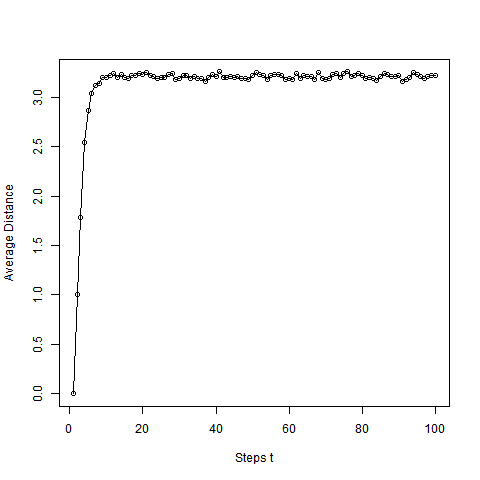
\includegraphics[width=.6\textwidth]{Q1b_1.png}
\caption{The average distance for random network with 1000 nodes}
\label{fig:p1_b1}
\end{figure}\\
\\
\begin{figure}[htbp]
\centering
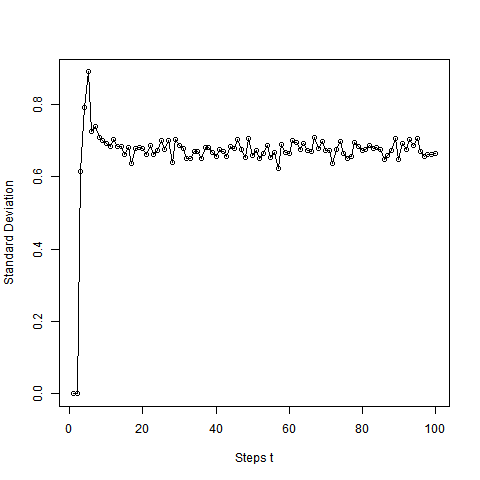
\includegraphics[width=.6\textwidth]{Q1b_2.png}
\caption{The standard deviation for random network with 1000 nodes}
\label{fig:p1_b2}
\end{figure}\\
\\
From the figures above, we can see that the average distance is around 3 and the standard deviation is about 0.7. As step t increases, these two values converge to the fixed value.

\subsection{Part c}
In theory, values of a random walker in d dimensional are $\langle s(t)\rangle=0$ and$\sqrt{\langle s^2(t)\rangle}$ = $\alpha \propto $t. However, the results in our random network are totally different from the theorical values. The standard deviation does not show any linear relationship with the number of steps t and average distance is not equal to zero. In fact, what we get in the random network, is that both the standard deviation and average distance converge to a constant.\\
\\
As for the different result of average distance, this is due to the mechanism of our random walk algorithm: the distance of first step is adding one, after that, the minimum value of distance that the walker can ever achieve is zero (due to the fact that we cannot have signed distance). As the distance is always nonnegative, the average value cannot reach zero.\\
\\
As for the different result of standard deviation, this is due to the structure of random network. We can see that the diameter is rather small in our random network which possible could make the nodes' distribution relatively seperate. The limited number of edges can not guarantee the walker can randomly walk in a widely distributed pattern. The result we get seems that at first $\sqrt{\langle s^2(t)\rangle}$ = $\alpha \propto $t, but later the random walker fell into a cluster and began walking in the local region.

\subsection{Part d}
When the number of nodes n is set to be 100, $\sigma^2(t)=\langle (s(t)-\langle s(t)\rangle)^2\rangle$ v.s. $t$ is plotted in Figure \ref{fig:p1_d1} and \ref{fig:p1_d2} respectively. And we choose 100 random walkers, and 100 as the maximum steps in order to get a better simulation result.
\begin{figure}[htbp]
\centering
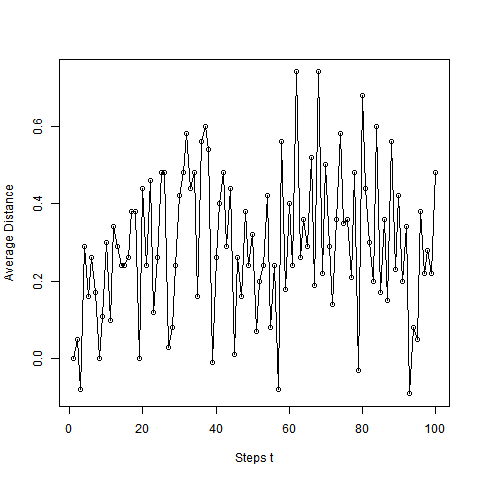
\includegraphics[width=.6\textwidth]{Q1d_1_100.png}
\caption{The average distance for random network with 100 nodes}
\label{fig:p1_d1}
\end{figure}

\begin{figure}[htbp]
\centering
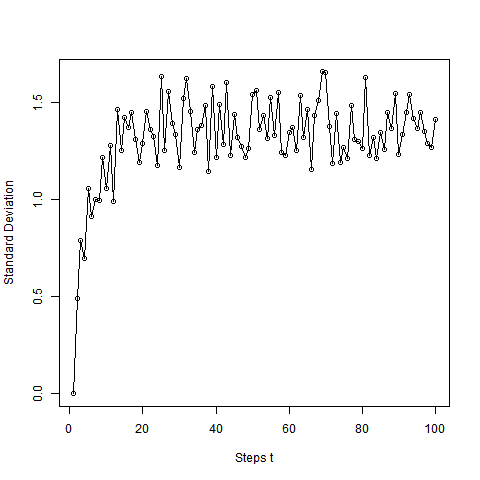
\includegraphics[width=.6\textwidth]{Q1d_2_100.png}
\caption{The standard deviation for random network with 100 nodes}
\label{fig:p1_d2}
\end{figure}
\noindent When the number of nodes n is set to be 10000, $\sigma^2(t)=\langle (s(t)-\langle s(t)\rangle)^2\rangle$ v.s. $t$ is plotted in Figure \ref{fig:p1_d3} and \ref{fig:p1_d4} respectively. And we choose 1000 random walkers, and 100 as the maximum steps in order to get a better simulation result.
\begin{figure}[htbp]
\centering
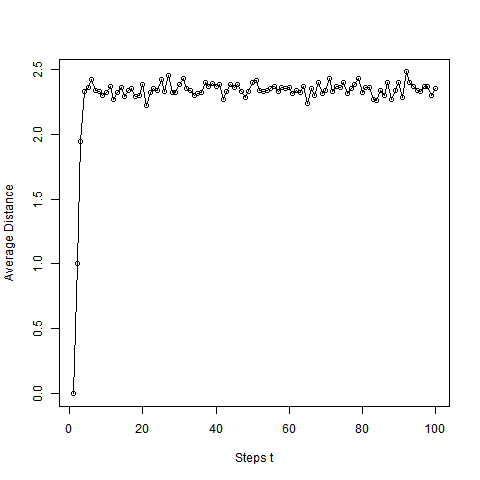
\includegraphics[width=.6\textwidth]{Q1d_1_10000.png}
\caption{The average distance for random network with 10000 nodes}
\label{fig:p1_d3}
\end{figure}\\
\\
\begin{figure}[htbp]
\centering
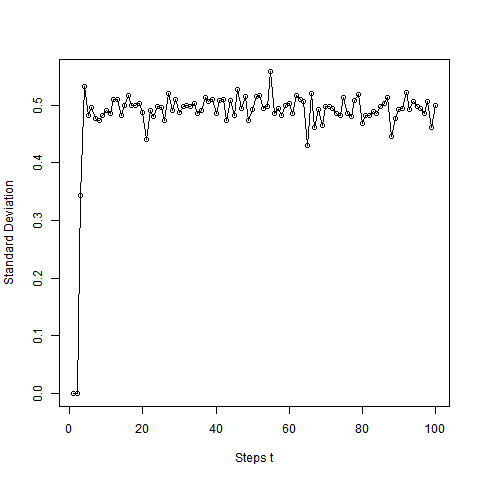
\includegraphics[width=.6\textwidth]{Q1d_2_10000.png}
\caption{The standard deviation for random network with 10000 nodes}
\label{fig:p1_d4}
\end{figure}\\
\\
The diameter of these three network is shown in Table \ref{tb:p1_d}.
\begin {table}[htbp]
\caption{diameter of random network}
\begin{adjustbox}{center}
\label{tb:p1_d}
\begin{tabular}{|c|c|c|c|}
\hline
\tabincell{c}{} & n=100 & n = 1000 & n = 10000\\
\hline
\tabincell{c}{diameter}& 9& 6 & 3\\
\hline

\end{tabular}
\end{adjustbox}
\end{table}
Comparing with Figure \ref{fig:p1_b1} and \ref{fig:p1_b2}, we can see the trend of  average distance and standard deviation in random network with  1000 and 10000 nodes are similar that both converge to constants. However, as the number of nodes increases(size of network increases), these two convergence values become smaller. This is because when the network becomes larger,the walker are freer to randomly walk in a relatively widely distributed pattern. Thus the average distance and the standard deviation will be more closer to the theorical values.\\
\\
Note that the diameter value for these networks decreases with smaller average distance and standard deviation as the number of nodes increase. Furthermore, the average distance can never exceed the value of its diameter. Thus, to some extent,the diameter plays a role in the properties of network.\\
\\
However, the random network with 100 nodes does not follow the same trend like the two other networks. This is possibly due to the fact that network with 100 nodes is disconnected and diameter is not applicable for disconnected graph. 

\subsection{Part e}
The degree distribution at the end of random walk is shown in Figure \ref{fig:p1_e1} and the degree distribution of the graph is shown in Figure \ref{fig:p1_e2}.\\

\begin{figure}[htbp]
\centering
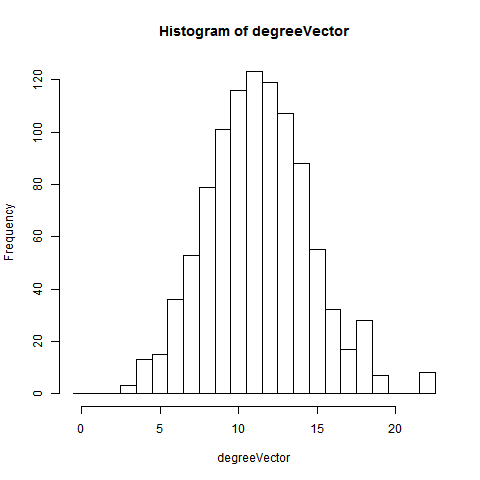
\includegraphics[width=.6\textwidth]{Q1e.png}
\caption{The degree distribution at the end of random walk}
\label{fig:p1_e1}
\end{figure}

\begin{figure}[htbp]
\centering
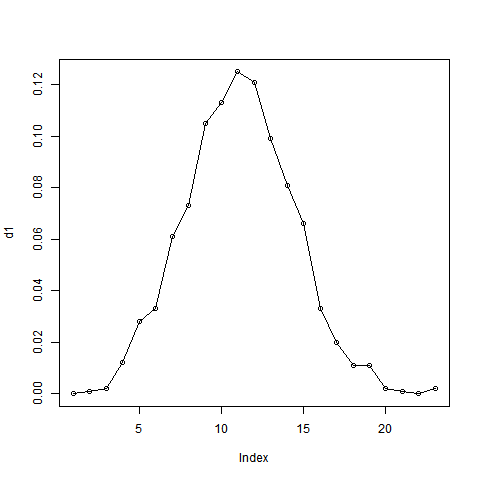
\includegraphics[width=.6\textwidth]{Q1a_1.png}
\caption{the degree distribution of the graph}
\label{fig:p1_e2}
\end{figure}
\noindent We can see from the figures above that the degree distribution at the end of the random walk and the degree distribution of graph are generally resembles each other.
This similarity between two distributions means that nodes the walker went through are randomized, thus indicates the reliability of our random walk algorithm.

\section{Problem2}\label{prob:p2}
In this part, we do random walk on networks with fat-tailed degree distribution
and try to analyze the relationship between random walk and network structure.

\subsection{Part a}
We create a fat-tailed network with 1000 nodes and degree distribution proportional to $x^{−3}$ by using the barabasi.game()function easily.

\subsection{Part b}
Similarly, we simulate the random walk process by assigning random number to neighborhood of certain node. And we choose 1000 random walkers, and 100 as the maximum steps in order to get a better simulation result. For each one random walkers, the start node is randomly choosen. In order to get the distance from each starting point at step t, we find the shortest paths between them and measure it. The average distance $\langle s(t)\rangle$, and standard deviation $\sigma^2(t)=\langle (s(t)-\langle s(t)\rangle)^2\rangle$ v.s. $t$ is plotted in Figure \ref{fig:p2_b1} and \ref{fig:p2_b2} respectively.
\begin{figure}[htbp]
\centering
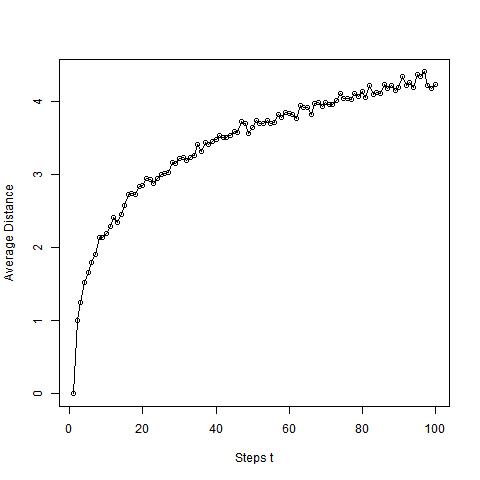
\includegraphics[width=.6\textwidth]{Q2b_1.png}
\caption{The average distance for fat-tailed network with 1000 nodes}
\label{fig:p2_b1}
\end{figure}\\
\\
\begin{figure}[htbp]
\centering
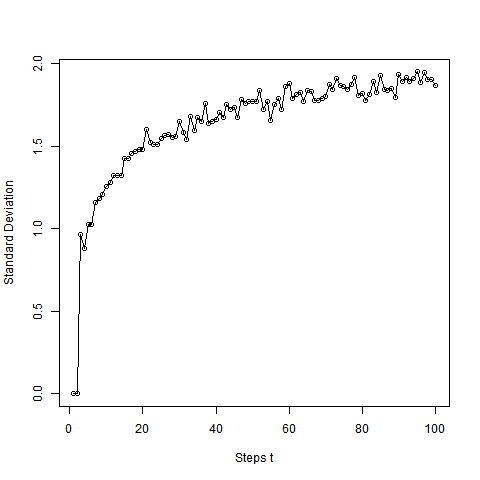
\includegraphics[width=.6\textwidth]{Q2b_2.png}
\caption{The standard deviation for fat-tailed network with 1000 nodes}
\label{fig:p2_b2}
\end{figure}\\
\\
From the figures above, we can see that the average distance and the standard deviation both grow proportional to the step t.


\subsection{Part c}
The results of average distance and standard deviation is different from the random network in problem 1. In the fat-tailed network, the degree distribution of the nodes is more tightly bounded and densely located in a small range, so the degree of each nodes is more likely resemble. Thus, with the incrementation of the step t, the walker will be more likely to walk in a remote area. In this case, the average distance and the the standard deviation will be proportional to the t.\\
\\
However, in the previous random network, the node is more sparsely distributed and the walk may be more likely to be ”trapped” in a certain area, which could be the reason the the convergence of these two indicators.\\
\\
The reason why the average distance still differs the theorical value zero is due to the mechanism of our random walk algorithm. The minimum value of distance that the walker can ever achieve is zero (due to the fact that we cannot have signed distance). As the distance is always nonnegative, the average value cannot reach zero.\\

\subsection{Part d}
When the number of nodes n is set to be 100, $\sigma^2(t)=\langle (s(t)-\langle s(t)\rangle)^2\rangle$ v.s. $t$ is plotted in Figure \ref{fig:p2_d1} and \ref{fig:p2_d2} respectively. And we choose 100 random walkers, and 100 as the maximum steps in order to get a better simulation result.
\begin{figure}[htbp]
\centering
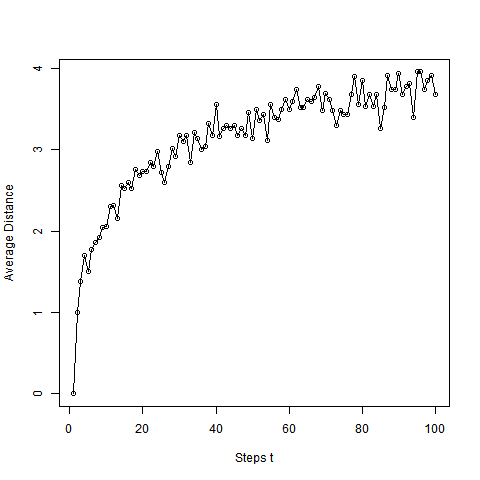
\includegraphics[width=.6\textwidth]{Q2d_1_100.png}
\caption{The average distance for fat-tailed network with 100 nodes}
\label{fig:p2_d1}
\end{figure}\\
\\
\begin{figure}[htbp]
\centering
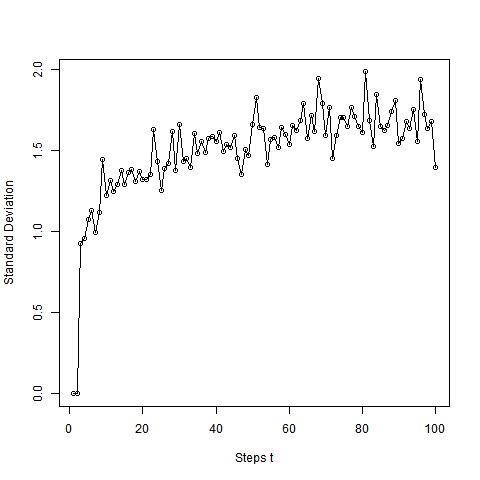
\includegraphics[width=.6\textwidth]{Q2d_2_100.png}
\caption{The standard deviation of average distance for fat-tailed with 100 nodes}
\label{fig:p2_d2}
\end{figure}\\
\\
When the number of nodes n is set to be 10000, $\sigma^2(t)=\langle (s(t)-\langle s(t)\rangle)^2\rangle$ v.s. $t$ is plotted in Figure \ref{fig:p2_d3} and \ref{fig:p2_d4} respectively. And we choose 10000 random walkers, and 100 as the maximum steps in order to get a better simulation result.
\begin{figure}[htbp]
\centering
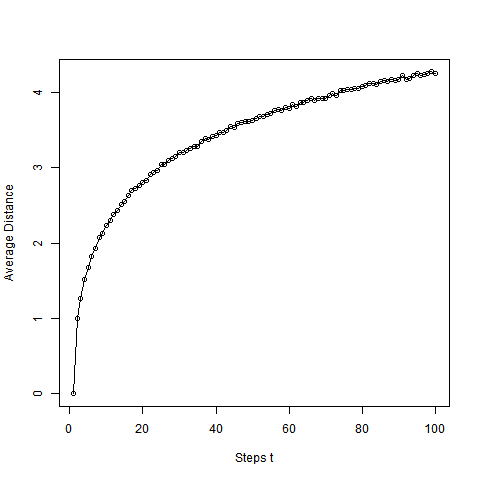
\includegraphics[width=.6\textwidth]{Q2d_1_10000.png}
\caption{The average distance for fat-tailed network with 10000 nodes}
\label{fig:p2_d3}
\end{figure}\\
\\
\begin{figure}[htbp]
\centering
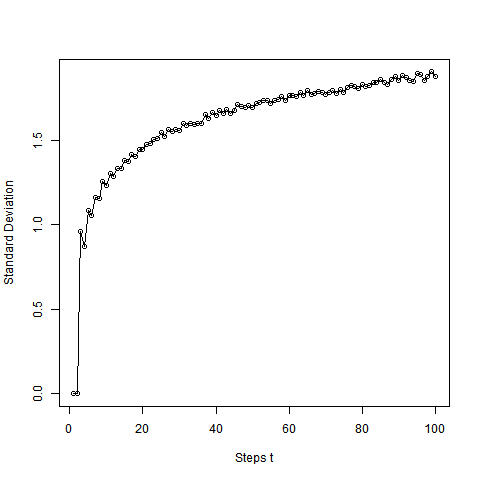
\includegraphics[width=.6\textwidth]{Q2d_2_10000.png}
\caption{The standard deviation of average distance for fat-tailed network with 10000 nodes}
\label{fig:p2_d4}
\end{figure}\\
\\
The diameter of these three networks is shown in Table \ref{tb:p2_d}.
\begin {table}[htbp]
\caption{diameter of fat-tailed network}
\begin{adjustbox}{center}
\label{tb:p2_d}
\begin{tabular}{|c|c|c|c|}
\hline
\tabincell{c}{} & n=100 & n = 1000 & n = 10000\\
\hline
\tabincell{c}{diameter}& 11 & 19 & 27\\
\hline

\end{tabular}
\end{adjustbox}
\end{table}
Comparing with Figure \ref{fig:p2_b1} and \ref{fig:p2_b2}, we can see the trend of  average distance and standard deviation in all three networks with  100, 1000 and 10000 nodes are similar that both proportional to t. Unlike 1(d), here 100 nodes fat-tailed network is connected, thus its result is similar to the other two and we can analyze these three results all together.\\
\\
Since every network is connected, the random walker can travel to any node in the network, then diameter will not play a role. Thus, the average distances among the three cases are nearly the same. However, the standard deviation in the case of 100 nodes is a bit larger than other two cases. This is  possibly due to the limited size in that case. If the network size is too small, walker are relatively easier to get trapped in certain subregion, thus the walker behavior becomes more uncertain.\\

\subsection{Part e}
The degree distribution at the end of random walk is shown in Figure \ref{fig:p2_e1} and the degree distribution of the graph is shown in Figure \ref{fig:p2_e2}.\\
\begin{figure}[htbp]
\centering
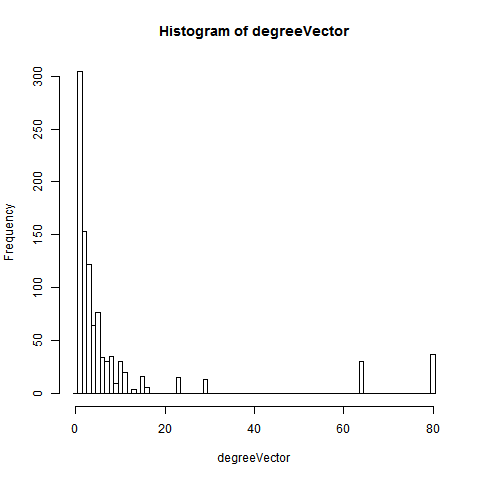
\includegraphics[width=.6\textwidth]{Q2e_1.png}
\caption{The degree distribution at the end of fat-tailed walk}
\label{fig:p2_e1}
\end{figure}

\begin{figure}[htbp]
\centering
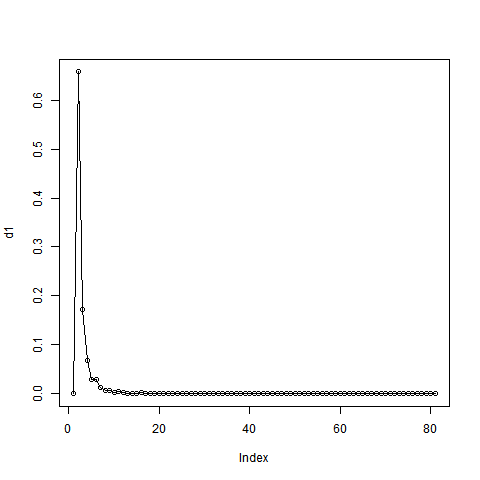
\includegraphics[width=.6\textwidth]{Q2a_1.png}
\caption{the degree distribution of the graph}
\label{fig:p2_e2}
\end{figure}
\noindent We can see from the figures above that the degree distribution at the end of the random walk and the degree distribution of graph are generally resembles each other.This similarity between two distributions means that nodes the walker went through are randomized, thus indicates the reliability of our random walk algorithm.

\section{Problem 4}
\subsection{Part a}
The ramdom directed network was created with the damping factor 0.85. It had 1000 nodes and we chose to run the random walk experiment for 1000 times. Figure \ref{fig:p4_a} shows the result of the average page rank.
\begin{figure}[htbp]
\centering
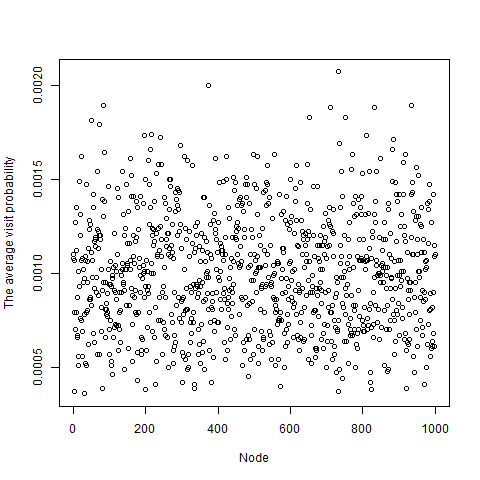
\includegraphics[width=.6\textwidth]{p4_a.png}
\caption{The page rank VS node index}
\label{fig:p4_a}
\end{figure}
\subsection{Part b}
The random directed network was created with the damping factor 0.85. It had 1000 nodes and we chose to run the random walk experiment for 1000 times. In this network, the walker has his own notion of interest, which means the teleportation probability to all nodes is not equal. Here, the teleportation probability is proportional to its pagerank. Figure \ref{fig:p4_b} shows the result of the average page rank for this personalized network.\\
\begin{figure}[htbp]
\centering
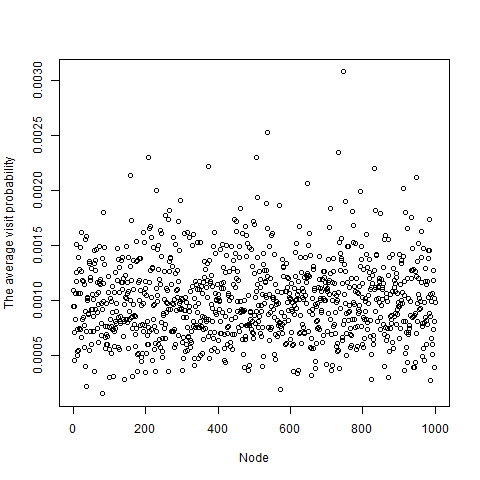
\includegraphics[width=.6\textwidth]{p4_b.png}
\caption{The personalized page rank VS node index}
\label{fig:p4_b}
\end{figure}
\\
Figure \ref{fig:p4_comp} shows the result when we put two kinds of pagerank together into one graph. From the figure we can see that due to the comparably large damping factor(0.85), there is no prominent difference between them. However, there are still some notable differences. For instance, some nodes have higher visit probability in personalized page rank than in normal page rank because teleportation probability is proportational to the original page rank which enlarge the effect of high page rank.
\begin{figure}[htbp]
\centering
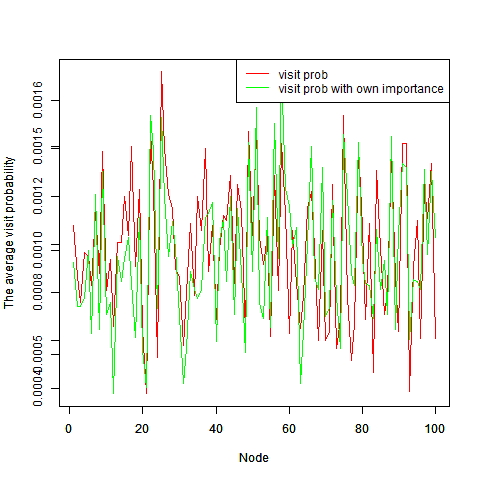
\includegraphics[width=.6\textwidth]{p4_compare.png}
\caption{Normal page rank VS Personalized page rank}
\label{fig:p4_comp}
\end{figure}

\subsection{Part c}
Taking into account the self-enforcement of the page rank, we need to add another factor to represent the users' random behavior. Thus, the page rank equation can be modified as
\begin{equation*}
PR(p_i) = d\sum_{p_j\in{M(p_i)}}\frac{PR(p_j)}{C(p_j)} + \frac{1-d}{N}
\end{equation*}
where $M(p_i)$ is the set of nodes that has links to $p_i$, $C(p_j)$ is the number of output links $p_j$ has, $N$ is the total number of nodes the network has, $d$ is the damping factor. This is the random-surfer model for page rank where the second factor represents the user may jump to a random page with the probability of $1-d$. It can avoid the problem of dangling page (values dissipates through pages without any links) and crawler trap(pages that just point to each other that all values may accumulate on those pages).
\end{document}